
\documentclass[letterpaper, 10 pt, conference]{ieeeconf}  % Comment this line out if you need a4paper

%\documentclass[a4paper, 10pt, conference]{ieeeconf}      % Use this line for a4 paper

\IEEEoverridecommandlockouts                           

\overrideIEEEmargins                                      % Needed to meet printer requirements.

%In case you encounter the following error:
%Error 1010 The PDF file may be corrupt (unable to open PDF file) OR
%Error 1000 An error occurred while parsing a contents stream. Unable to analyze the PDF file.
%This is a known problem with pdfLaTeX conversion filter. The file cannot be opened with acrobat reader
%Please use one of the alternatives below to circumvent this error by uncommenting one or the other
%\pdfobjcompresslevel=0
%\pdfminorversion=4

% See the \addtolength command later in the file to balance the column lengths
% on the last page of the document

% The following packages can be found on http:\\www.ctan.org
\usepackage{graphics} % for pdf, bitmapped graphics files
\usepackage{epsfig} % for postscript graphics files
\usepackage{mathptmx} % assumes new font selection scheme installed
\usepackage{times} % assumes new font selection scheme installed
\usepackage{tabularx}
\usepackage{graphicx}
\usepackage{amsmath}
\usepackage{amsfonts}
\usepackage{amssymb}
\usepackage{url}
\usepackage{cite}

\PassOptionsToPackage{hyphens}{url}
\usepackage{hyperref}

\title{\LARGE \bf
Multimodal Assessment of Well-Being in Alzheimer’s Disease Caregivers
}


\author{%
Junen Xiao$^{1}$, Akane Sano$^{1}$%
\thanks{$^{1}$Department of Electrical and Computer Engineering, Rice University, Houston, TX 77005, USA.}%
}

\begin{document}

\maketitle
\thispagestyle{empty}
\pagestyle{empty}


%%%%%%%%%%%%%%%%%%%%%%%%%%%%%%%%%%%%%%%%%%%%%%%%%%%%%%%%%%%%%%%%%%%%
\begin{abstract}
Spousal and family caregivers of people with Alzheimer’s disease and related dementias often experience elevated stress, burden, and loneliness, yet these states are usually measured with infrequent questionnaires. We examine whether multimodal data can support everyday assessment of caregiver well-being, using two caregiver studies (Project ACT, n = 43; Project CARE, n = 100) with Fitbit signals, ecological momentary assessment (EMA), smartphone sensing, and baseline background surveys. We classify high- versus low-risk caregivers on the Perceived Stress Scale (PSS), Zarit Burden Interview (ZBI), and UCLA Loneliness Scale (UCLALS), comparing a feature-engineered baseline with foundation-model embeddings and large language model (LLM) text representations under participant-level leave-one-out cross-validation. Preliminary results show that baseline context surveys reach AUCs of 0.76--0.86, whereas Fitbit-only features reach 0.43--0.46. Because some baseline scales resemble the target questions, we are screening them for target leakage before completing the multimodal experiments.
\end{abstract}


%%%%%%%%%%%%%%%%%%%%%%%%%%%%%%%%%%%%%%%%%%%%%%%%%%%%%%%%%%%%%%%%%%%%%%%%%%%%%%%%
\section{INTRODUCTION}
Caring for a person with Alzheimer's disease and related dementias (AD/ADRD) is a major source of chronic psychological strain. In the United States, nearly 13 million family members and friends provided unpaid care in 2025, contributing more than 19 billion hours, and 59\% of them reported high or very high emotional stress \cite{alz2026}. These dimensions of strain unfold on different time scales: perceived stress \cite{cohen1983} responds to daily demands, caregiver burden \cite{gratao2019} accumulates over months, and loneliness \cite{russell1996} reflects a more persistent sense of social disconnection. Yet all three are typically measured with a questionnaire administered once, which cannot show how a caregiver's state changes from day to day.

Wearables and ecological momentary assessment (EMA) can observe these daily dynamics. Machine learning on wearable data has been used to detect daily-life stress \cite{smets2018}. Passively sensed smartphone and Fitbit data, together with EMA, have likewise been used to predict short-term symptom changes in people with multiple sclerosis \cite{xia2025}. Among caregivers, disrupted circadian rhythms have been associated with burden \cite{park2025}, and in-home sensors have been used to classify it \cite{chimehi2026}. However, prior work mostly targets a single construct, often outside caregiving populations. It also leaves open how much each source contributes: heart rate and sleep reflect physiology, EMA captures momentary mood and fatigue, background surveys describe more stable characteristics such as depressive symptoms and grief, and smartphone sensing (location and screen use) may capture mobility and daily routines that a wrist-worn device misses.

How to represent these data is a second open question. Engineered features are interpretable but may discard information, and EMA responses, some of which are conditionally activated, are awkward to encode as tables. Time-series and wearable foundation models, such as MOMENT \cite{goswami2024moment} and LSM-2 \cite{xu2025lsm2}, learn reusable embeddings and can handle recordings with gaps, while large language models (LLMs) can convert EMA responses and participant profiles into text representations \cite{kim2024healthllm,xu2024mentalllm}. Whether these representations help in small caregiver cohorts is unknown.

We study these questions in two caregiver cohorts, Project ACT ($n=43$, one 7-day session) and Project CARE ($n=100$, three 7-day sessions), which pair minute-level Fitbit data, EMA, and background surveys, plus smartphone sensing for a subset, with the PSS, ZBI, and UCLALS collected after each session. Our contributions are:
\begin{itemize}
    \item We classify high- versus low-risk caregivers on each scale, comparing a feature-engineered baseline with foundation-model embeddings and LLM text representations under participant-level leave-one-out cross-validation.
    \item We quantify through source ablations which of Fitbit, EMA, and background context contributes most to each scale, and, in an exploratory analysis on the subset of participants with phone data, whether smartphone sensing adds predictive value.
    \item We use the repeated sessions in CARE to test whether within-person changes in sensor data track changes in outcomes.
\end{itemize}
\begin{figure}[t]
    \centering
    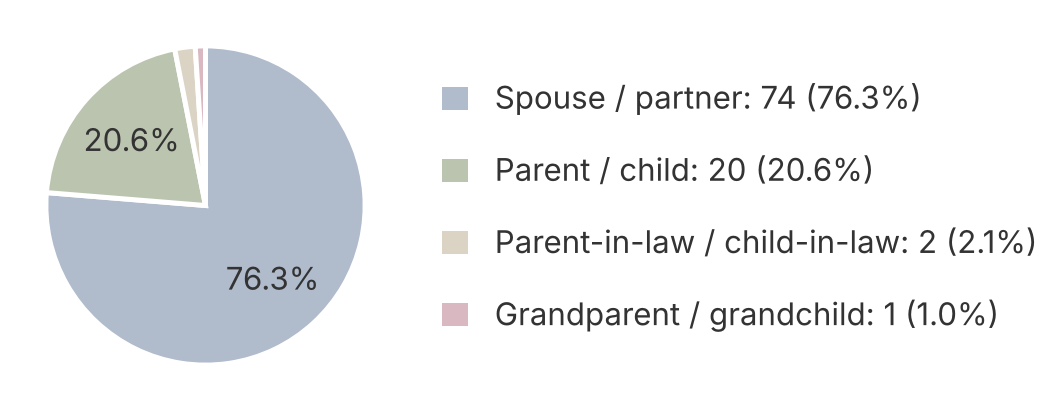
\includegraphics[width=\columnwidth]{relationship.png}
    \caption{Relationship between caregivers and care recipients ($n=97$).}
    \label{fig:relationship}
\end{figure}

\begin{table}[t]
\centering
\caption{Binary classification rules and label distribution for psychological scales ($n=97$).}
\label{tab:label_distribution}
\begin{tabular}{lccc}
\hline
\textbf{Scale} & \textbf{Binary Rule} & \textbf{Low Risk (n,\%)} & \textbf{High Risk (n,\%)} \\
\hline
PSS~\cite{cohen1983} & $\geq 14 \rightarrow 1$ & 29 (29.90\%) & 68 (70.10\%) \\
UCLALS~\cite{russell1996} & $\geq 35 \rightarrow 1$ & 30 (30.93\%) & 67 (69.07\%) \\
ZBI~\cite{gratao2019} & $\geq 21 \rightarrow 1$ & 25 (25.77\%) & 72 (74.23\%) \\
\hline
\end{tabular}
\end{table}

\begin{figure*}[!t]
  \centering
  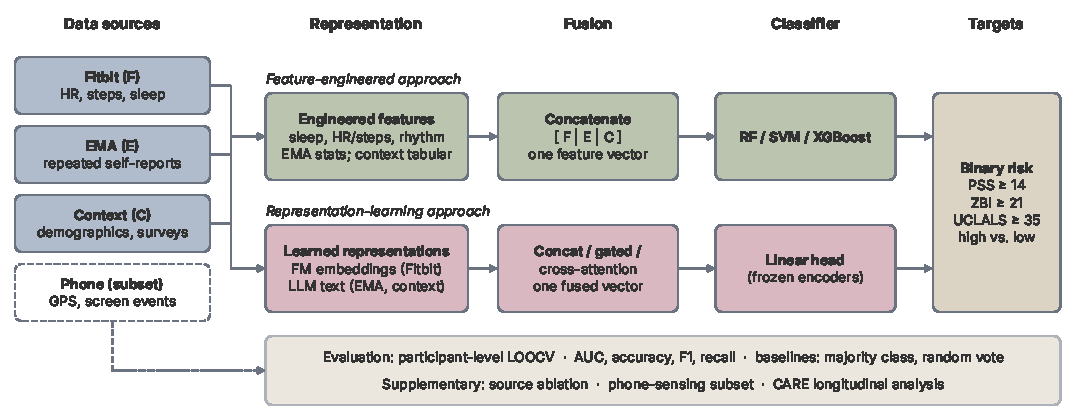
\includegraphics[width=0.9\textwidth]{workflow.pdf}
  \caption{Overview of the two modeling pipelines. Fitbit, EMA, and baseline context
  are converted into engineered features (top) or learned representations (bottom),
  fused, and classified into high vs.\ low risk for PSS, ZBI, and UCLALS. Phone
  sensing is used only in a separate subset study.}
  \label{fig:workflow}
\end{figure*}
\section{Method}

\subsection{Study Cohorts, Data, and Labels}
Data come from two caregiver studies, Project ACT and Project CARE, which enrolled 43 and 100 caregivers of people with Alzheimer's disease and related dementias, respectively. ACT participants completed one 7-day session and CARE participants completed three. The analytic sample comprises 97 caregivers with Fitbit data, EMA, and all three target scales (mean age 65 years; 88\% women; 86\% White). Most were spouses or partners of the care recipient (Fig.~\ref{fig:relationship}).

During each session, participants wore a Fitbit that recorded minute-level heart rate and step counts, and sleep status during sleep periods. They also answered brief EMA surveys: a morning sleep-quality item once a day, and several random prompts per day on mood, fatigue, helping, and social interactions. A subset of participants also had smartphone data collected with the AWARE framework~\cite{ferreira2015aware}, which passively logged GPS location and timestamped screen-status events. Because phone data reduce the available sample (48 participants have both Fitbit and phone data), we treat phone sensing as a subset analysis. At study start, caregivers completed baseline surveys (e.g., anticipatory grief, comorbidities, depressive symptoms, and partner responsiveness) and a demographic questionnaire.

After each session, participants completed the Perceived Stress Scale (PSS)~\cite{cohen1983}, Zarit Burden Interview (ZBI)~\cite{gratao2019}, and UCLA Loneliness Scale (UCLALS)~\cite{russell1996}, which served as ground-truth labels. We binarized each scale using established cut-offs into high- and low-risk groups. The rules and label distributions are summarized in Table~\ref{tab:label_distribution}.


\subsection{Features and Representations}
We process each data source separately and describe how they are combined in the next subsection (Fig.~\ref{fig:workflow}).

\textit{Baseline context.} Background context comprises demographics and baseline surveys on, for example, anticipatory grief, comorbidities, depressive symptoms, and partner responsiveness. In the baseline pipeline these are used directly as tabular features. Because some baseline scale items resemble the outcome questions, we screen these scales for target leakage before final modeling. We also plan to have large language models (LLMs; GPT, Gemini, and Llama) select the key background information and write a concise profile for each participant, following the practice of giving LLMs text-formatted inputs for health prediction~\cite{kim2024healthllm}. Where clinical notes are available, we will additionally use retrieval-augmented generation~\cite{lewis2020rag} to retrieve relevant psychological information and generate a clinical-style summary. % TODO: confirm clinical notes exist for this cohort; if not, delete this sentence

\textit{EMA.} EMA responses are summarized per session as means, within-person variability, and time-of-day patterns. Because some EMA questions are conditionally activated and do not fit a fixed table, we will also convert the responses into text with table-to-text models and encode the text into fixed-length vectors. % TODO: confirm which text encoder is used

\textit{Fitbit.} We compute sleep features (durations of asleep, restless, and awake states and the Sleep Regularity Index~\cite{fischer2021sri}), daily heart-rate and step statistics by time of day, and circadian rhythm features (M10/L5~\cite{goncalves2014}, cosinor parameters~\cite{cornelissen2014}, and deviations from a 24-hour template~\cite{tseng2020}). We also plan to embed the raw time series with pretrained foundation models, MOMENT~\cite{goswami2024moment} and SensorFM~\cite{sensorfm2026}, and compare these embeddings with the engineered features.

\textit{Phone sensing.} Smartphone location and screen-status data are available only for a subset of participants, so we do not include them in the main pipeline. Instead, we summarize them as daily location and screen-use features and add them to the models in a separate subset study. % TODO: confirm which phone features are computed

\subsection{Models and Evaluation}
\begin{figure*}[!t]
  \centering
  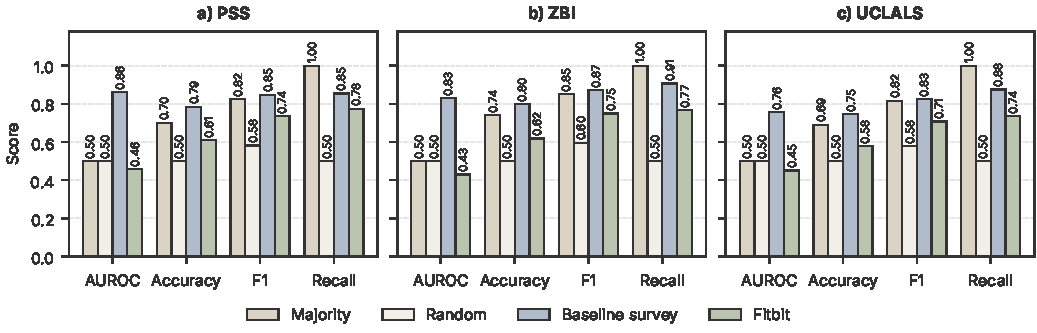
\includegraphics[width=0.9\textwidth]{results_single.pdf}
  \caption{Performance of the majority-class and random baselines and of logistic regression models using baseline survey or Fitbit features for PSS, ZBI, and UCLALS risk classification.}
  \label{fig:results}
\end{figure*}
\textit{Baselines.} We use two simple reference baselines for the three binary targets (PSS, ZBI, and UCLALS). The majority-class baseline assigns every participant to the most frequent class in the training data, and the probabilistic random baseline samples predictions from the training class distribution. These matter here because 69--74\% of participants are high-risk (Table~\ref{tab:label_distribution}), so a classifier that always predicts high risk already reaches a similar accuracy. % TODO: if the random baseline is averaged over repeated runs, say so

\textit{Feature-engineered approach.} Engineered Fitbit, EMA, and context features are concatenated into a single feature vector and classified with Random Forest~\cite{breiman2001}, support vector machine~\cite{cortes1995}, or XGBoost~\cite{chen2016xgboost} models.

\textit{Representation-learning approach.} Frozen foundation-model embeddings (Fitbit) and LLM-based text representations (EMA and context) are combined with three fusion strategies, namely concatenation, gated fusion, and cross-attention~\cite{vaswani2017}, and a linear classification head is trained on top of the frozen encoders.

\textit{Evaluation.} All models use participant-level leave-one-out cross-validation: in each fold, all sessions of one participant are held out, so sessions from the same person never appear in both training and test sets. Predictions from all folds are pooled to compute AUC, accuracy, F1, and recall.

\textit{Supplementary analyses.} We run three additional experiments: (i) a source ablation using Fitbit only, EMA only, or baseline context only, to identify which source contributes most; (ii) a subset study that adds phone sensing for participants who have it; and (iii) a longitudinal analysis of CARE participants with all three sessions, testing whether changes in sensor data track changes in outcomes.

\section{Results}

Fig.~\ref{fig:results} compares the two reference baselines with logistic regression models trained on baseline survey or Fitbit features alone. Because 69--74\% of participants are high-risk, the majority-class baseline already reaches an accuracy of 0.69--0.74 and an F1 of 0.82--0.85, while the random baseline sits near 0.50 on AUROC, accuracy, and recall. The baseline survey model beats both on all three targets, with AUROC of 0.76--0.86 and accuracy of 0.75--0.80, although its accuracy gain over the majority class is small (e.g., 0.79 vs.\ 0.70 for PSS). The Fitbit-only model performs worse than the majority class (accuracy 0.58--0.62) and below chance in AUROC (0.43--0.46), and adding Fitbit to the survey also lowered AUROC (e.g., 0.86 to 0.70 for PSS). Because some survey scales resemble the outcome questions, the survey results may be inflated by target leakage, which we are still screening for.


\section{Discussion}
Baseline survey features were the only input that clearly beat the reference baselines, whereas Fitbit features alone did not. Background scales such as anticipatory grief describe a caregiver's psychological state directly, while a week of Fitbit data captures daily routine, which may relate only weakly to longer-term stress, burden, or loneliness. The survey results should be read as a reference rather than evidence for passive sensing, since some scale items resemble the outcome questions and target leakage may inflate them. A Fitbit AUROC below 0.5 more likely reflects noise and overfitting than a real inverse relationship, which may also explain why adding Fitbit to the survey lowered performance.

These results are preliminary, and the models are a first pass. Next, we will test whether richer Fitbit rhythm features, foundation-model embeddings, EMA, and fusion improve on the survey-only reference, and whether the phone-sensing subset and CARE longitudinal analysis add signal.


\section*{Acknowledgements}
This work was supported by the National Institutes of Health (NIH) under Grant Nos. R01AG062690, K25AG070306, and R01DA059925, and by the National Science Foundation (NSF) under Grant Nos. 1840167 and 2047296. The research was conducted under the supervision of Professor Akane Sano.

\section*{CRediT Author Statement}
Junen Xiao: Methodology, Software, Formal Analysis, Writing. Akane Sano: Supervision, Funding Acquisition.

\section*{Code Availability}
The LaTeX source code of this report, including all files and figures required is available at:

\href{https://github.com/PepperJess99/ELEC-594/tree/main/Spring%202026/Midterm%20Report}{GitHub repository}

\addtolength{\textheight}{-12cm}   % This command serves to balance the column lengths
                                  % on the last page of the document manually. It shortens
                                  % the textheight of the last page by a suitable amount.
                                  % This command does not take effect until the next page
                                  % so it should come on the page before the last. Make
                                  % sure that you do not shorten the textheight too much.

%%%%%%%%%%%%%%%%%%%%%%%%%%%%%%%%%%%%%%%%%%%%%%%%%%%%%%%%%%%%%%%%%%%%%%%%%%%%%%%%



%%%%%%%%%%%%%%%%%%%%%%%%%%%%%%%%%%%%%%%%%%%%%%%%%%%%%%%%%%%%%%%%%%%%%%%%%%%%%%%%
\bibliographystyle{ieeetr}

\bibliography{reference}


\end{document}